%=============================================================================
%  FINAL YEAR PROJECT REPORT (PFA) -- AI-Based Intrusion Detection System
%  Master SDIA -- Data Science and Artificial Intelligence
%  ENSA El Jadida -- Chouaib Doukkali University
%=============================================================================
\documentclass[12pt, a4paper]{report}

%--- Encoding, Font & Language ------------------------------------------------
\usepackage[utf8]{inputenc}
\usepackage[T1]{fontenc}

% Times New Roman -- required by PFA template (Times New Roman body + math)
\usepackage{newtxtext}
\usepackage{newtxmath}

\usepackage[french]{babel}
\setlength{\headheight}{15pt}

%--- Page Layout -- PFA template: 2.5 cm margins, 3 cm left (binding) ---------
\usepackage[top=2.5cm, bottom=2.5cm, left=3cm, right=2.5cm]{geometry}
\usepackage{setspace}
\onehalfspacing
\setlength{\parskip}{4pt plus 1pt minus 1pt}
\setlength{\parindent}{0pt}

%--- Mathematics --------------------------------------------------------------
\usepackage{amsmath, bm}

%--- Figures & Tables ---------------------------------------------------------
\usepackage{graphicx}
\usepackage{float}
\usepackage{subcaption}
\usepackage{booktabs}
\usepackage{multirow}
\usepackage{array}
\usepackage{tabularx}
\PassOptionsToPackage{table,xcdraw}{xcolor}
\usepackage{xcolor}
\usepackage{colortbl}

%--- Source Code --------------------------------------------------------------
\usepackage{listings}

\definecolor{codegray}{rgb}{0.95,0.95,0.95}
\definecolor{codegreen}{rgb}{0.0,0.5,0.0}
\definecolor{codepurple}{rgb}{0.4,0.0,0.6}
\definecolor{codeblue}{rgb}{0.0,0.0,0.7}

\lstdefinestyle{pythonstyle}{
  backgroundcolor=\color{codegray},
  commentstyle=\color{codegreen}\itshape,
  keywordstyle=\color{codeblue}\bfseries,
  stringstyle=\color{codepurple},
  basicstyle=\ttfamily\small,
  breakatwhitespace=false,
  breaklines=true,
  captionpos=b,
  keepspaces=true,
  numbers=left,
  numberstyle=\tiny\color{gray},
  numbersep=8pt,
  showspaces=false,
  showstringspaces=false,
  showtabs=false,
  tabsize=2,
  language=Python,
  frame=single,
  rulecolor=\color{gray!40},
  xleftmargin=1.5em,
  framexleftmargin=1.5em
}
\lstset{style=pythonstyle}

% Rename the auto-generated listings list title
\renewcommand{\lstlistlistingname}{Liste des Codes}

%--- Colors (kept for info boxes; headings are black per PFA template) ---------
\definecolor{mainblue}{RGB}{31,56,100}
\definecolor{accentblue}{RGB}{46,117,182}
\definecolor{lightgray}{RGB}{242,242,242}
\definecolor{darkgray}{RGB}{64,64,64}
\definecolor{successgreen}{RGB}{0,128,0}
\definecolor{warnorange}{RGB}{204,85,0}

%--- Headers & Footers -- PFA template style ----------------------------------
\usepackage{fancyhdr}
\pagestyle{fancy}
\fancyhf{}
\fancyhead[L]{\small\textit{\leftmark}}
\fancyhead[R]{\small\thepage}
\fancyfoot[C]{}
\renewcommand{\headrulewidth}{0.4pt}
\renewcommand{\footrulewidth}{0pt}

% First page of each chapter: page number centered at bottom
\fancypagestyle{plain}{%
  \fancyhf{}%
  \fancyfoot[C]{\thepage}%
  \renewcommand{\headrulewidth}{0pt}%
  \renewcommand{\footrulewidth}{0pt}%
}

%--- Chapter & Section Titles -- PFA Template Style ---------------------------
\usepackage{titlesec}

% Chapter: 22pt, Bold, UPPERCASE, centered, black (sz=44 half-pts in template)
\titleformat{\chapter}[display]
  {\normalfont\fontsize{22}{26}\bfseries\centering}
  {\MakeUppercase{\chaptertitlename}\ \thechapter}{6pt}{\MakeUppercase}
\titlespacing*{\chapter}{0pt}{0pt}{18pt}

% Section: 14pt, Bold, black, numbered (sz=28 half-pts = 14pt in template)
\titleformat{\section}
  {\normalfont\fontsize{14}{17}\bfseries}
  {\thesection}{1em}{}
\titlespacing*{\section}{0pt}{14pt plus 2pt minus 2pt}{6pt}

% Subsection: 12pt, Bold, black, numbered
\titleformat{\subsection}
  {\normalfont\fontsize{12}{14}\bfseries}
  {\thesubsection}{1em}{}
\titlespacing*{\subsection}{0pt}{10pt plus 2pt minus 2pt}{4pt}

% Subsubsection: 12pt, Bold Italic, black
\titleformat{\subsubsection}
  {\normalfont\fontsize{12}{14}\bfseries\itshape}
  {\thesubsubsection}{1em}{}

%--- Hyperlinks -- black links for print (PFA convention) ---------------------
\usepackage[colorlinks=true,
            linkcolor=black,
            citecolor=black,
            urlcolor=mainblue,
            pdftitle={Rapport de Mini Projet -- Deep Learning},
            pdfauthor={EL MAHDI BOUDERNA, Yassine Mounabih, Yassine EL Hattab}]{hyperref}

%--- Note Boxes -- plain black horizontal-rule style (no color fill) ----------
\usepackage{tcolorbox}
\tcbuselibrary{skins,breakable}

% Plain style: only top + bottom black rules, white background, bold title
\tcbset{notestyle/.style={
  enhanced,
  breakable,
  colback=white,
  colframe=black,
  leftrule=0pt,
  rightrule=0pt,
  toprule=0.8pt,
  bottomrule=0.8pt,
  arc=0pt,
  outer arc=0pt,
  fonttitle=\bfseries,
  coltitle=black,
  attach title to upper={\par\smallskip},
}}

% All three variants render identically in plain black
\newtcolorbox{infoblue}[1][]{notestyle, title={#1}}
\newtcolorbox{infogreen}[1][]{notestyle, title={#1}}
\newtcolorbox{infoorange}[1][]{notestyle, title={#1}}



%--- Miscellaneous ------------------------------------------------------------
\usepackage{enumitem}
\usepackage{caption}
\captionsetup{font=small, labelfont=bf, format=hang}
\usepackage{tikz}

%--- Acronyms -----------------------------------------------------------------
\usepackage{acronym}

%=============================================================================
\begin{document}
% Langue: Français
\hypersetup{pageanchor=false}

%--- Page de Garde -- Modèle Professionnel de Mini Projet ---------------------
\begin{titlepage}
\thispagestyle{empty}
\centering

% Ligne des logos
\begin{minipage}[t]{0.35\textwidth}
  \flushleft
  
\includegraphics[height=2.0cm]{ucd.png}
\end{minipage}%
\hfill%
\begin{minipage}[t]{0.35\textwidth}
  \flushright
  
\includegraphics[height=2.0cm]{ensa.png}
\end{minipage}

\vspace{0.4cm}

% Noms de l'université et de l'école
{\fontsize{13}{15}\bfseries\MakeUppercase{Université Chouaib Doukkali}}\\[0.15cm]
{\fontsize{12}{14}\bfseries École Nationale des Sciences Appliquées -- El Jadida}\\[0.10cm]
{\fontsize{10}{12} Département de Génie Informatique}\\[0.05cm]
{\fontsize{10}{12}\itshape Master en Sciences des Données et Intelligence Artificielle (SDIA)}

\vspace{0.4cm}
\noindent\rule{\linewidth}{1.5pt}\\[0.25cm]
{\fontsize{15}{18}\bfseries\MakeUppercase{Rapport de Mini Projet}}\\[0.15cm]
{\fontsize{12}{14}\bfseries Module : Deep Learning}\\[0.20cm]
\noindent\rule{\linewidth}{1.5pt}

\vspace{0.8cm}

% Boîte du titre du projet
\begin{center}
  \setlength{\fboxsep}{15pt}
  \framebox[\linewidth]{
    \begin{minipage}{0.9\linewidth}
      \centering
      \fontsize{15}{18}\bfseries
      Système de Détection d'Intrusion\\
      Basé sur l'Intelligence Artificielle\\[10pt]
      \fontsize{10.5}{13}\normalfont\itshape
      Une Étude Comparative sur NSL-KDD et CSE-CIC-IDS2018 :\\
      Apprentissage Automatique Classique, Apprentissage Profond (CNN, BiLSTM, MLP),\\
      et Architectures d'Ensemble Hybrides
    \end{minipage}
  }
\end{center}

\vfill

% Bloc des auteurs et du superviseur
\noindent
\begin{minipage}[t]{0.48\textwidth}
  \flushleft
  {\fontsize{11}{13}\selectfont\textbf{Réalisé par :}}\\[0.15cm]
  {\fontsize{10.5}{12}\selectfont
  EL MAHDI BOUDERNA\\
  Yassine Mounabih\\
  Yassine EL Hattab}
\end{minipage}
\hfill
\begin{minipage}[t]{0.48\textwidth}
  \flushright
  {\fontsize{11}{13}\selectfont\textbf{Encadré par :}}\\[0.15cm]
  {\fontsize{10.5}{12}\selectfont
  Prof. Youness Abouqora}
\end{minipage}

\vfill
\noindent\rule{\linewidth}{1.5pt}\\[0.15cm]
{\fontsize{11}{13}\bfseries Année Universitaire : 2025 -- 2026}\\[0.15cm]
\noindent\rule{\linewidth}{1.5pt}

\end{titlepage}
\clearpage
\hypersetup{pageanchor=true}

%--- Front matter: Roman page numbering ----------------------------------------
\pagenumbering{roman}

%--- Table des Matières, Figures, Tableaux -------------------------------------
\tableofcontents
\clearpage
\addcontentsline{toc}{chapter}{\listfigurename}
\listoffigures
\clearpage
\addcontentsline{toc}{chapter}{\listtablename}
\listoftables

%--- List of Acronyms ---------------------------------------------------------
\clearpage
\chapter*{Liste des Acronymes}
\addcontentsline{toc}{chapter}{Liste des Acronymes}

\begin{acronym}[XGBoost]  % longest acronym sets column width
  \acro{AI}{Artificial Intelligence}
  \acro{AUC}{Area Under the (ROC) Curve}
  \acro{BiLSTM}{Bidirectional Long Short-Term Memory}
  \acro{CIC}{Canadian Institute for Cybersecurity}
  \acro{CNN}{Convolutional Neural Network}
  \acro{DDoS}{Distributed Denial of Service}
  \acro{DL}{Deep Learning}
  \acro{DoS}{Denial of Service}
  \acro{F1}{F1-Score (harmonic mean of Precision and Recall)}
  \acro{FN}{False Negative}
  \acro{FP}{False Positive}
  \acro{IDS}{Intrusion Detection System}
  \acro{KDD}{Knowledge Discovery and Data Mining}
  \acro{KNN}{K-Nearest Neighbours}
  \acro{LightGBM}{Light Gradient Boosting Machine}
  \acro{LSTM}{Long Short-Term Memory}
  \acro{ML}{Machine Learning}
  \acro{MLP}{Multilayer Perceptron}
  \acro{NIDS}{Network Intrusion Detection System}
  \acro{NSL-KDD}{Network Security Laboratory -- Knowledge Discovery and Data Mining dataset}
  \acro{PFA}{Projet de Fin d'Année (Final Year Project)}
  \acro{RF}{Random Forest}
  \acro{RNN}{Recurrent Neural Network}
  \acro{ROC}{Receiver Operating Characteristic}
  \acro{SDIA}{Science des Données et Intelligence Artificielle (Data Science and Artificial Intelligence)}
  \acro{SHAP}{SHapley Additive exPlanations}
  \acro{SMOTE}{Synthetic Minority Over-sampling Technique}
  \acro{SVM}{Support Vector Machine}
  \acro{XGBoost}{eXtreme Gradient Boosting}
\end{acronym}

%--- Switch to Arabic page numbering from Chapter 1 onward -------------------
\clearpage
\pagenumbering{arabic}

%=============================================================================
\chapter*{Introduction Générale}
\addcontentsline{toc}{chapter}{Introduction Générale}
\label{chap:intro}
%=============================================================================

La transformation numérique des sociétés modernes a fondamentalement modifié le paysage des menaces pesant sur la sécurité de l'information. Les secteurs des infrastructures critiques, des systèmes financiers à la santé, s'appuient sur des environnements en réseau exposés à des activités adverses sophistiquées, notamment les menaces persistantes avancées (APT), les failles zero-day, les campagnes de déni de service distribué (DDoS) et l'exfiltration furtive de données.

Les \textbf{Systèmes de Détection d'Intrusion (IDS)} représentent une ligne de défense indispensable. Les approches basées sur les signatures sont fondamentalement réactives (incapables d'identifier les nouvelles menaces), ce qui oriente la recherche vers la détection d'anomalies à l'aide de l'apprentissage automatique. Le domaine est passé des méthodes d'ensemble classiques aux architectures d'apprentissage profond capables de capturer des interactions complexes de caractéristiques, facilitées par des benchmarks réalistes à grande échelle tels que CSE-CIC-IDS2018 \cite{sharafaldin2018}.

Ce projet de fin d'année, réalisé au sein du Master SDIA de l'ENSA El Jadida, poursuit les objectifs suivants :

\begin{itemize}[leftmargin=2em]
  \item Évaluer huit algorithmes classiques d'apprentissage automatique pour la détection d'intrusion binaire sur NSL-KDD ;
  \item Implémenter et évaluer trois architectures d'apprentissage profond (BiLSTM, CNN 1D, MLP) sur les deux jeux de données ;
  \item Étendre l'évaluation à CSE-CIC-IDS2018, un problème à dix classes avec plus d'un million d'échantillons ;
  \item Concevoir et évaluer deux architectures d'ensemble hybrides par jeu de données ;
  \item Analyser l'impact du déséquilibre des classes et l'effet de l'étalonnage du seuil de décision.
\end{itemize}

Le rapport est organisé comme suit. Le chapitre~\ref{chap:etat_art} passe en revue l'état de l'art. Le chapitre~\ref{chap:datasets} décrit les deux jeux de données et leur prétraitement. Le chapitre~\ref{chap:ml} couvre les résultats de l'apprentissage automatique classique. Le chapitre~\ref{chap:dl} couvre l'apprentissage profond, les architectures hybrides et une analyse comparative exhaustive de tous les modèles. Le chapitre~\ref{chap:general_conclusion} conclut avec les principales découvertes et les perspectives d'avenir.

%=============================================================================
\chapter{État de l'Art}
\label{chap:etat_art}
%=============================================================================

\section{Paradigmes de Détection}

Un système de détection d'intrusion réseau (NIDS) distingue globalement deux paradigmes. \textbf{La détection par signature} confronte les événements à des modèles d'attaques connus—très précis pour les menaces cataloguées mais inefficaces contre les attaques zero-day. \textbf{La détection par anomalie} construit un modèle de comportement normal et signale les déviations ; bien que capable de détecter de nouvelles attaques, elle génère des taux de faux positifs plus élevés. Les architectures IDS hybrides combinent les deux, utilisant la correspondance de signatures comme premier filtre et la détection d'anomalies pour le trafic résiduel.

\section{Apprentissage Automatique Classique pour les IDS}

Les méthodes d'ensemble basées sur les arbres dominent la littérature des IDS pour les données réseau tabulaires. Les \textbf{Forêts Aléatoires (Random Forests)} réduisent la variance grâce à l'agrégation bootstrap. Les \textbf{Machines d'Amplification de Gradient (Gradient Boosting Machines)} corrigent itérativement les erreurs résiduelles, excellant sur les modèles d'attaques subtils. \textbf{XGBoost} et \textbf{LightGBM} accélèrent l'amplification de gradient avec une construction d'arbres basée sur des histogrammes. Des études antérieures ont révélé que RF et XGBoost apparaissent dans plus de 60 \% des systèmes IDS les plus performants. Les SVM restent compétitifs sur des jeux de données de taille modérée mais sont prohibitivement lents sur des données de l'ordre du million d'enregistrements en raison d'une complexité de $\mathcal{O}(n^2)$--$\mathcal{O}(n^3)$.

\section{Architectures d'Apprentissage Profond pour les IDS}

Les \textbf{CNN 1D}, conçus à l'origine pour la reconnaissance d'images, ont démontré une extraction robuste de caractéristiques à partir de flux réseau tabulaires en traitant le vecteur de caractéristiques comme un signal 1D. Leur efficacité en termes de paramètres grâce au partage des poids permet une détection efficace des corrélations locales de caractéristiques.

Les \textbf{réseaux LSTM} sont théoriquement adaptés aux données séquentielles. Le LSTM bidirectionnel (BiLSTM) traite les séquences dans les deux sens pour un contexte plus riche. Cependant, lorsque les flux réseau sont représentés comme des \emph{agrégats statistiques}—comme dans NSL-KDD et CSE-CIC-IDS2018—les LSTM ajoutent une charge de calcul sans avantage représentationnel par rapport aux CNN ou aux MLP.

Des modèles \textbf{basés sur les Transformers} ont récemment été appliqués aux IDS avec des plongements contextuels améliorant la détection de catégories d'attaques à faible fréquence, mais exigent beaucoup plus de ressources de calcul.

\section{Ensembles Hybrides et Jeux de Données de Référence}

Les ensembles hétérogènes surpassent systématiquement les classificateurs uniques : empiler XGBoost avec les sorties d'un réseau neuronal réduit à la fois les taux de faux positifs et de faux négatifs. Deux jeux de données occupent des positions centrales dans la littérature récente :

\begin{itemize}
  \item \textbf{NSL-KDD} \cite{tavallaee2009} : Corrige la redondance de KDD Cup 1999. Malgré son ancienneté, il reste le benchmark le plus utilisé en raison de sa petite taille et de ses propriétés bien comprises.
  \item \textbf{CSE-CIC-IDS2018} \cite{sharafaldin2018} : Généré par l'Institut Canadien pour la Cybersécurité (CIC) sur sept jours dans une topologie d'entreprise réaliste. Son ampleur ($>$16M d'enregistrements) et sa diversité le rendent plus représentatif que les anciens benchmarks.
\end{itemize}

La littérature souligne systématiquement trois défis : \textbf{le déséquilibre des classes} (traité par la pondération des classes, SMOTE et l'étalonnage des seuils) ; \textbf{la généralisation} à travers les environnements réseau ; et \textbf{l'interprétabilité} via les outils d'IA explicable (XAI) comme SHAP et LIME.

%=============================================================================
\chapter{Jeux de Données et Prétraitement}
\label{chap:datasets}
%=============================================================================

\section{Jeu de Données NSL-KDD}

Introduit par Tavallaee et al.\ en 2009 \cite{tavallaee2009}, NSL-KDD remédie à deux lacunes de KDD Cup 1999 : la suppression des doublons et la sélection des enregistrements stratifiée par difficulté. Chaque enregistrement décrit une connexion TCP/IP avec \textbf{41 caractéristiques} (propriétés de la connexion, caractéristiques de contenu dérivées de la charge utile et statistiques de trafic temporelles), étiquetée comme normale ou l'un des 39 sous-types d'attaques regroupés en quatre familles (DoS, Probe, R2L, U2R). La composition du jeu de données et la distribution des classes sont présentées dans le Tableau~\ref{tab:nslkdd_comp} et la Figure~\ref{fig:nsl_attack_dist}.

\begin{table}[H]
\centering
\caption{Composition du jeu de données NSL-KDD}
\label{tab:nslkdd_comp}
\begin{tabular}{lccc}
\toprule
\textbf{Sous-ensemble} & \textbf{Enregistrements} & \textbf{Normal} & \textbf{Attaques} \\
\midrule
KDDTrain+ & 125,973 & 67,343 (53,5\%) & 58,630 (46,5\%) \\
KDDTest+  & 22,544  & 9,711 (43,1\%)  & 12,833 (56,9\%) \\
\bottomrule
\end{tabular}
\end{table}

\begin{figure}[H]
  \centering
  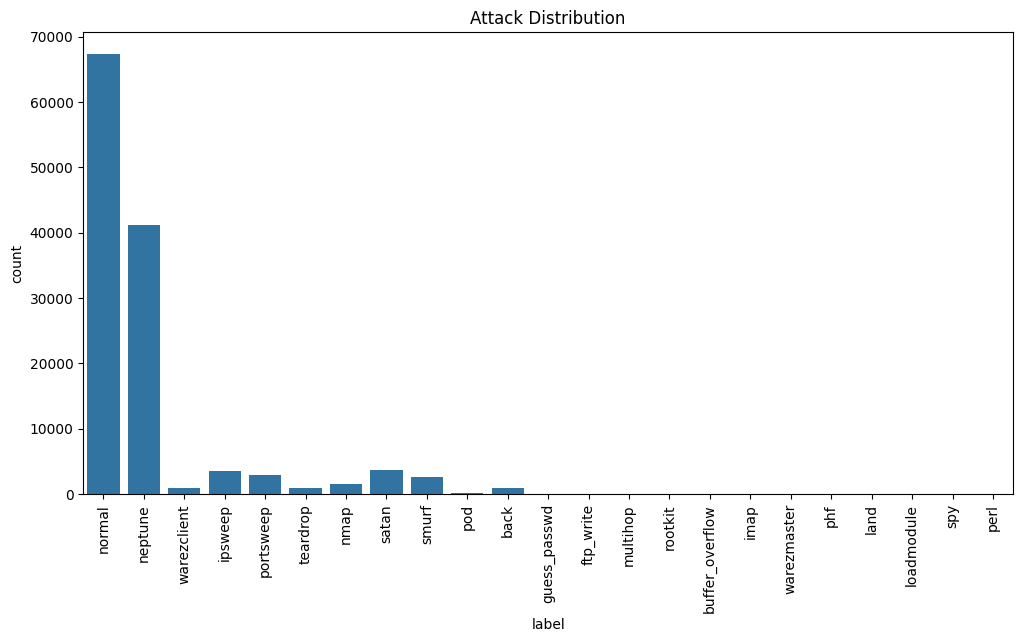
\includegraphics[width=0.85\textwidth]{figures/attack_distribution.png}
  \caption{Distribution des types d'attaques dans l'ensemble d'apprentissage de NSL-KDD}
  \label{fig:nsl_attack_dist}
\end{figure}

\textbf{Pipeline de prétraitement :} Tous les sous-types d'attaques sont mappés vers une seule classe d'attaque (binaire). La colonne \texttt{difficulty} est supprimée pour éviter toute fuite de données. Les caractéristiques catégorielles (\texttt{protocol\_type}, \texttt{service}, \texttt{flag}) sont encodées par labels pour les modèles basés sur les arbres et avec l'encodage one-hot pour les modèles d'apprentissage profond, étendant le vecteur à $\approx$122 caractéristiques. Toutes les caractéristiques numériques sont standardisées (moyenne nulle, variance unitaire) à l'aide d'un scaler ajusté exclusivement sur les données d'entraînement. Pour l'apprentissage profond, les entrées sont remodelées en $(samples,\ features,\ 1)$ pour le CNN ou en $(samples,\ 1,\ features)$ pour le BiLSTM.

\section{Jeu de Données CSE-CIC-IDS2018}

Publié par l'Institut Canadien pour la Cybersécurité \cite{sharafaldin2018}, ce jeu de données a été généré sur sept jours consécutifs dans un réseau d'entreprise contrôlé (50 machines attaquantes, 420 machines victimes). Les fichiers PCAP bruts ont été traités en \textbf{77 caractéristiques numériques de flux} via CICFlowMeter, couvrant la durée des flux, les temps d'inter-arrivée, les statistiques de longueur de paquet, le nombre d'indicateurs (flags) et les débits. Le jeu de données comprend 15 types d'attaques distincts répartis en six familles (Tableau~\ref{tab:cic_attacks_full}).

\begin{table}[H]
\centering
\caption{Distribution du trafic dans CSE-CIC-IDS2018}
\label{tab:cic_attacks_full}
\small
\begin{tabularx}{\textwidth}{@{}>{\raggedright\arraybackslash}p{2.4cm} X >{\raggedleft\arraybackslash}p{2.0cm}@{}}
\toprule
\textbf{Famille} & \textbf{Types d'Attaques} & \textbf{Volume} \\
\midrule
Benign & Trafic normal & 5,329,008 \\
DDoS & DDoS-LOIC-HTTP, DDOS-HOIC, DDOS-LOIC-UDP & 775,955 \\
DoS & DoS-Hulk, DoS-GoldenEye, DoS-Slowloris, DoS-SlowHTTPTest & 196,568 \\
Brute Force & SSH-Bruteforce, FTP-BruteForce, Brute Force-Web, Brute Force-XSS & 94,898 \\
Bot & Bot & 144,535 \\
Infiltration & Infiltration & 118,483 \\
Web Attacks & SQL Injection, Brute Force-XSS & 85 \\
\bottomrule
\end{tabularx}
\end{table}

\begin{figure}[H]
  \centering
  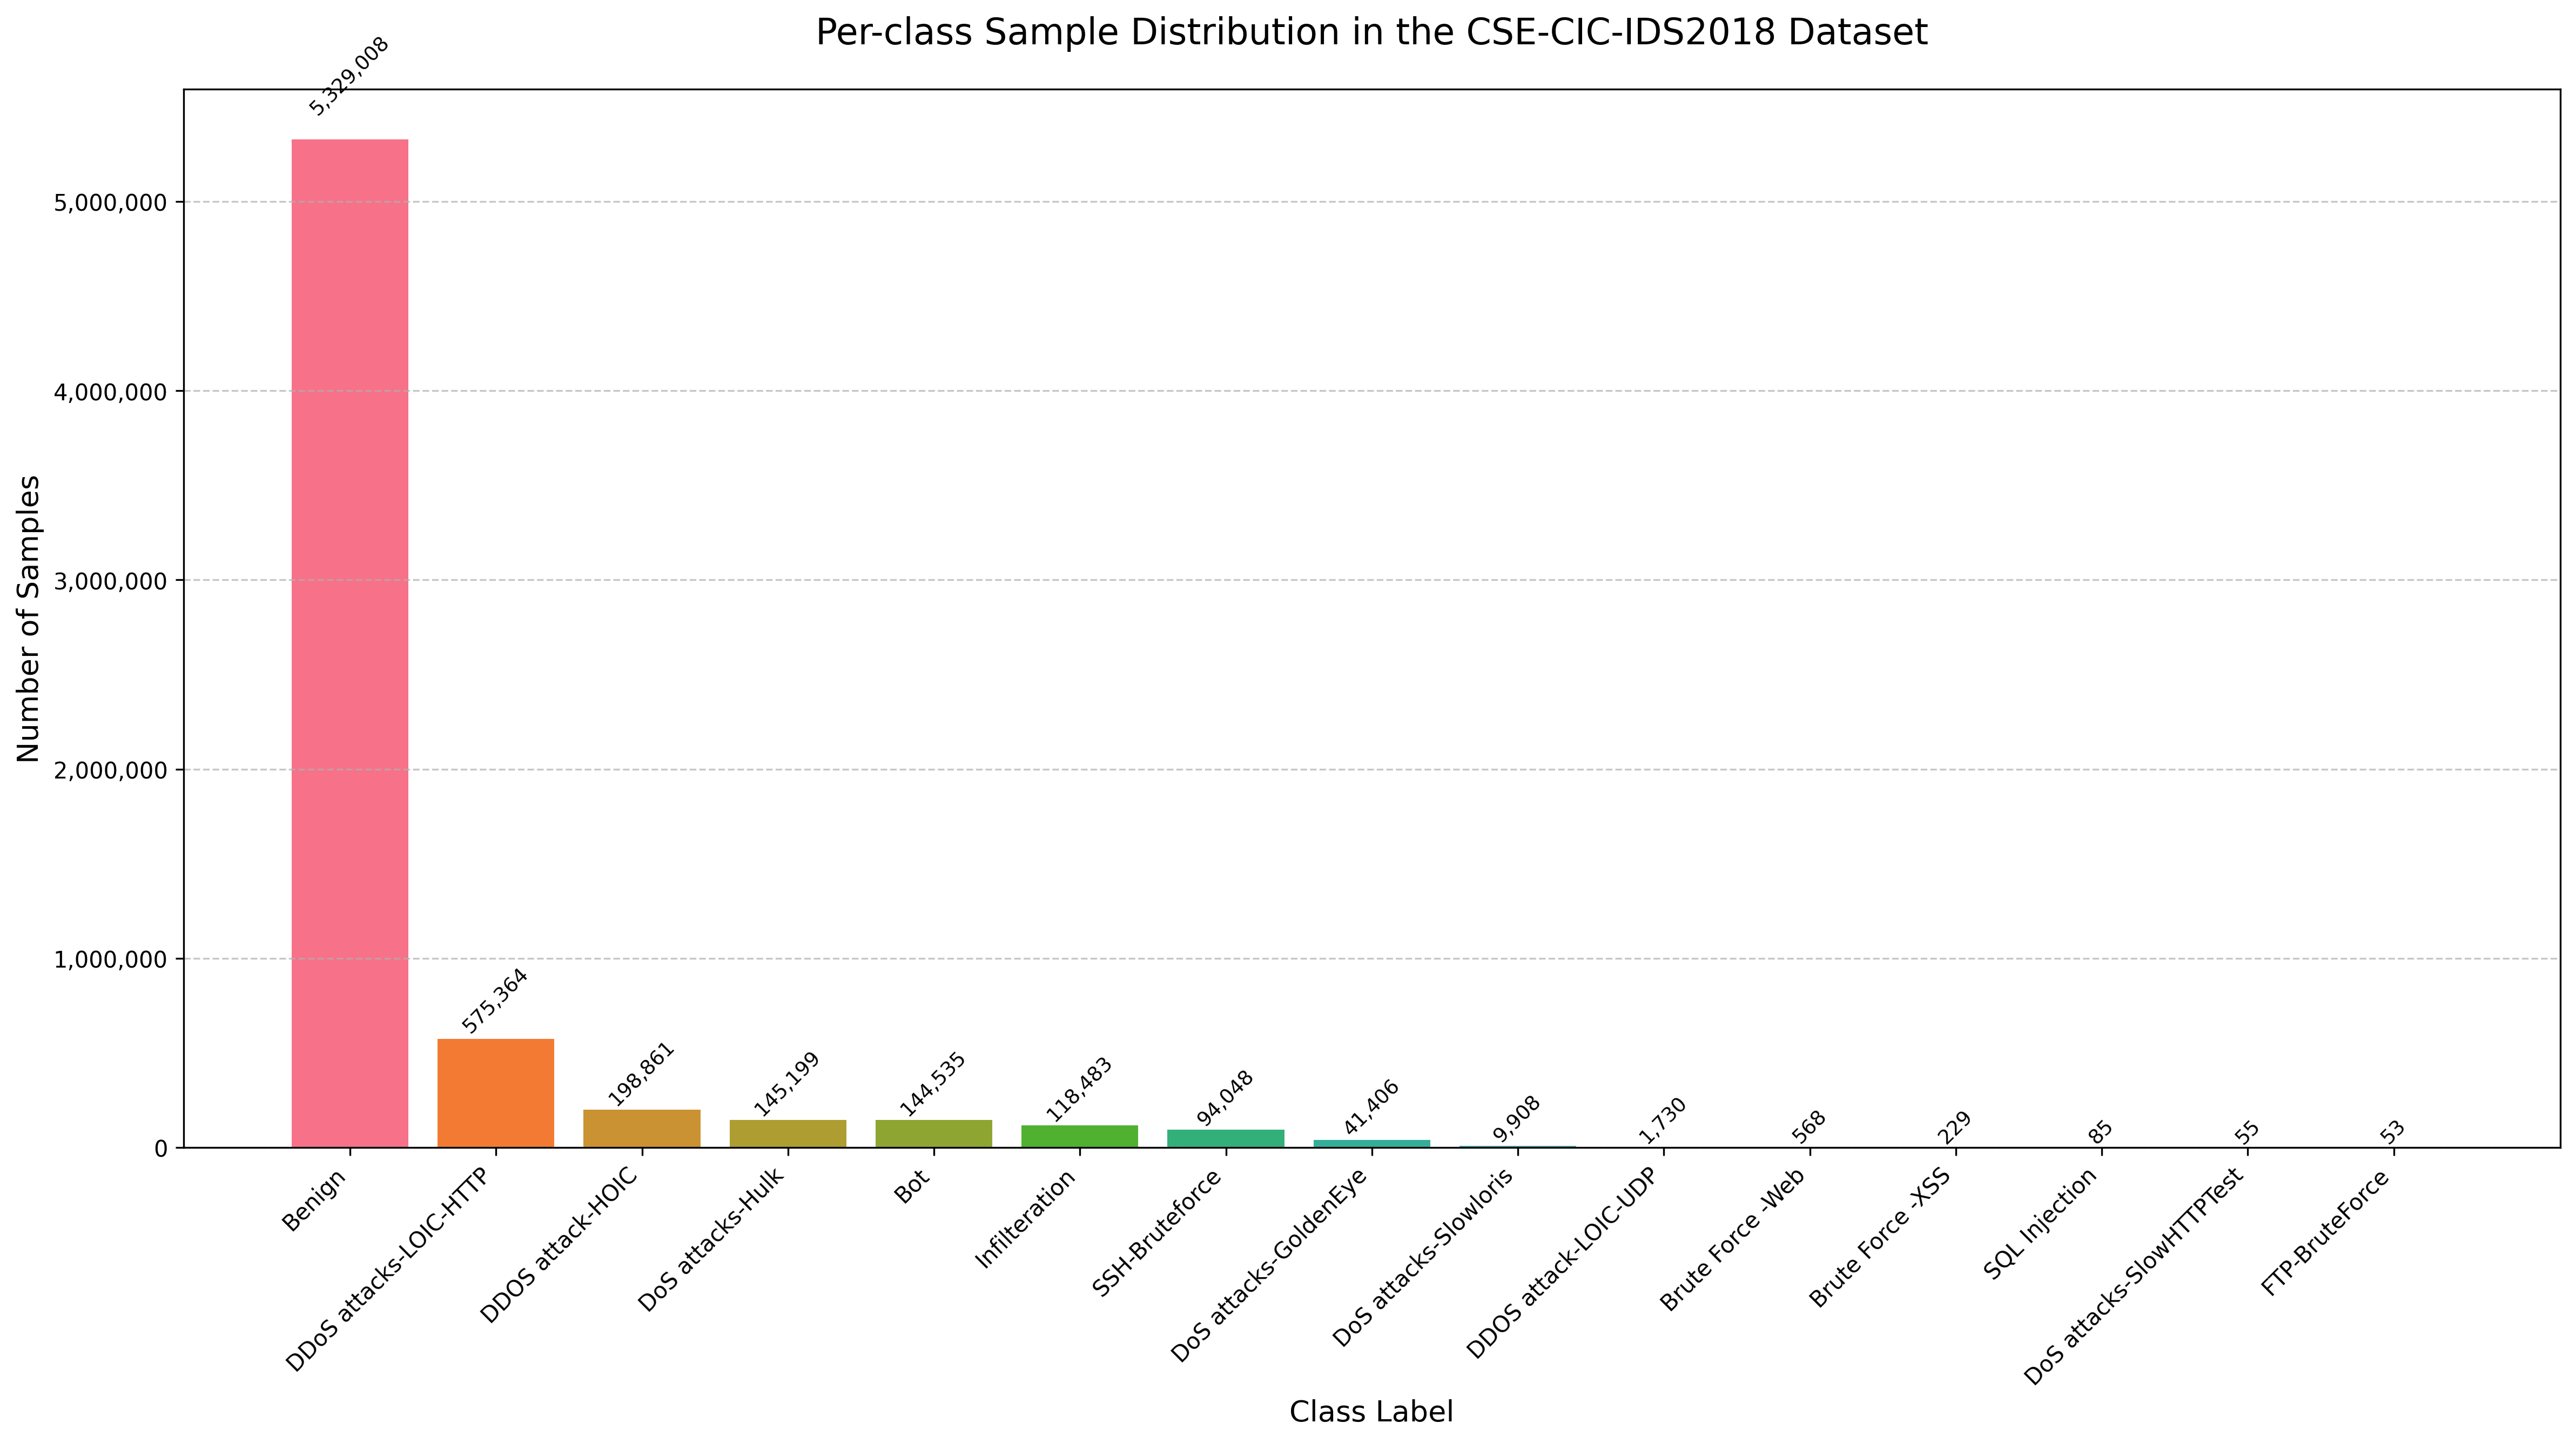
\includegraphics[width=0.85\textwidth]{figures/cic_class_distribution.png}
  \caption{Distribution des échantillons par classe dans le jeu de données CSE-CIC-IDS2018}
  \label{fig:cic_class_dist}
\end{figure}

\textbf{Pipeline de prétraitement :} Le jeu de données est distribué sous forme de fichiers Parquet. Après la concaténation, la colonne \texttt{Timestamp} est supprimée et les valeurs infinies/NaN sont nettoyées. Les données sont sous-échantillonnées à 1 000 000 d'enregistrements pour faciliter le calcul. Cinq classes d'attaques avec moins de 100 échantillons post-sous-échantillonnage (SQL Injection, DoS-SlowHTTPTest, FTP-BruteForce, Brute Force-Web, Brute Force-XSS) sont supprimées, ce qui donne un problème à \textbf{10 classes}. Les données sont réparties 70/15/15 (entraînement/validation/test) avec un échantillonnage stratifié. La standardisation des caractéristiques suit la même approche (ajustement sur l'entraînement uniquement) que pour NSL-KDD. Les poids équilibrés des classes sont calculés comme $w_c = N / (K \cdot n_c)$, et plafonnés pour prévenir l'instabilité due aux classes très rares.

%=============================================================================
\chapter{Expériences d'Apprentissage Automatique Classique}
\label{chap:ml}
%=============================================================================

\section{Modèles et Configurations}

Sur \textbf{NSL-KDD}, huit classificateurs supervisés ont été évalués pour la classification binaire (Tableau~\ref{tab:nsl_ml_params}). Sur \textbf{CSE-CIC-IDS2018}, trois méthodes d'ensemble extensibles (Forêt Aléatoire, XGBoost, LightGBM) ont été évaluées dans des configurations de base et avec réglage d'hyperparamètres sur un sous-échantillon de 300 000 enregistrements (Tableau~\ref{tab:cic_ml_params}).

\begin{table}[H]
\centering
\caption{Configurations des modèles d'apprentissage automatique classique pour NSL-KDD}
\label{tab:nsl_ml_params}
\small
\begin{tabular}{ll}
\toprule
\textbf{Modèle} & \textbf{Paramètres Clés} \\
\midrule
Random Forest          & \texttt{n\_estimators=100} \\
Decision Tree          & Critère de Gini, profondeur non restreinte \\
SVM                    & Noyau RBF, $C=1$ \\
KNN                    & $k=5$, distance euclidienne \\
Logistic Regression    & \texttt{max\_iter=2000}, solveur lbfgs \\
Naive Bayes (Gaussian) & Distribution gaussienne par caractéristique \\
AdaBoost               & \texttt{n\_estimators=100}, taux d'apprentissage 1.0 \\
Gradient Boosting      & \texttt{n\_estimators=100}, \texttt{lr=0.1} \\
\bottomrule
\end{tabular}
\end{table}

\begin{table}[H]
\centering
\caption{Configurations des modèles d'ensemble pour CSE-CIC-IDS2018}
\label{tab:cic_ml_params}
\small
\begin{tabularx}{\textwidth}{l >{\raggedright\arraybackslash}X >{\raggedright\arraybackslash}X}
\toprule
\textbf{Modèle} & \textbf{Base} & \textbf{Ajusté (Tuned)} \\
\midrule
Random Forest
    & \texttt{n\_est=200, depth=20}
    & \texttt{n\_est=300, depth=25, balanced\_subsample} \\
\midrule
XGBoost
    & \texttt{n\_est=500, depth=6, lr=0.05}
    & Régularisation accrue ($\gamma=2$, $\lambda=3$) \\
\midrule
LightGBM
    & \texttt{n\_est=500, depth=8, lr=0.05}
    & \texttt{n\_est=1000, lr=0.03, min\_child=20} \\
\bottomrule
\end{tabularx}
\end{table}

\section{Résultats sur NSL-KDD}

Le Tableau~\ref{tab:nsl_ml_full} présente les métriques complètes pour les huit classificateurs. Gradient Boosting atteint la plus grande précision (\textbf{80,6 \%}) et le meilleur score F1 (\textbf{0,800}), mais son rappel de 0,682 signifie qu'il manque environ 32 \% de toutes les attaques—un biais systématique de faux négatifs qui justifie les stratégies hybrides et d'étalonnage des seuils.

\begin{table}[H]
\centering
\caption{Résultats de l'apprentissage automatique classique sur KDDTest+ (classification binaire)}
\label{tab:nsl_ml_full}
\begin{tabular}{lcccc}
\toprule
\textbf{Modèle} & \textbf{Précision globale} & \textbf{Précision (Precision)} & \textbf{Rappel (Recall)} & \textbf{F1} \\
\midrule
\rowcolor{lightgray}
Gradient Boosting   & \textbf{0,806} & 0,968 & 0,682 & \textbf{0,800} \\
Decision Tree       & 0,792 & 0,963 & 0,623 & 0,756 \\
AdaBoost            & 0,790 & 0,964 & 0,657 & 0,781 \\
SVM (RBF)           & 0,782 & 0,976 & 0,633 & 0,768 \\
Random Forest       & 0,781 & 0,965 & 0,607 & 0,745 \\
Naive Bayes         & 0,771 & 0,911 & 0,663 & 0,768 \\
KNN ($k$=5)         & 0,768 & 0,971 & 0,610 & 0,749 \\
Logistic Regression & 0,754 & 0,925 & 0,618 & 0,741 \\
\bottomrule
\end{tabular}
\end{table}

\begin{figure}[H]
  \centering
  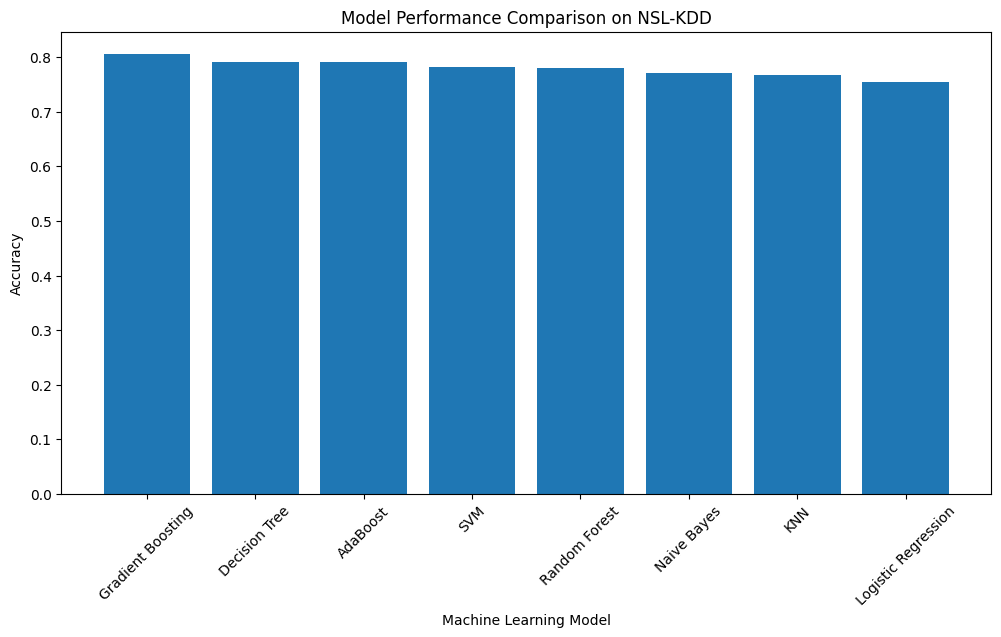
\includegraphics[width=0.85\textwidth]{figures/ml_accuracy_bar.png}
  \caption{Précision et scores F1 des modèles classiques sur NSL-KDD}
  \label{fig:nsl_ml_bar}
\end{figure}

\begin{figure}[H]
  \centering
  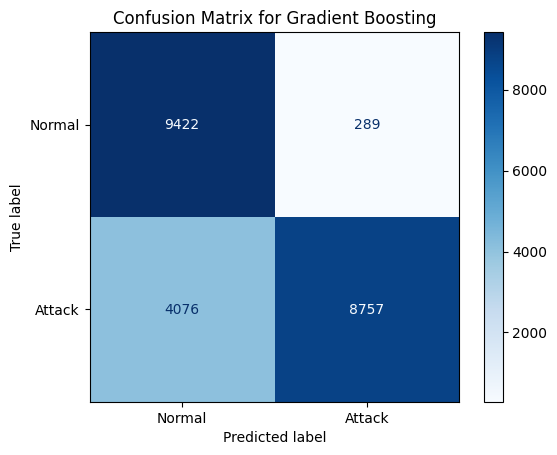
\includegraphics[width=0.55\textwidth]{figures/cm_gradient_boosting.png}
  \caption{Matrice de confusion du classificateur Gradient Boosting sur NSL-KDD}
  \label{fig:nsl_cm_gb}
\end{figure}

\section{Résultats sur CSE-CIC-IDS2018}

L'ajustement des hyperparamètres apporte des améliorations substantielles (Tableau~\ref{tab:cic_ml_results}). La Forêt Aléatoire (Random Forest) ajustée atteint \textbf{94,80 \%} de précision (+4,65 points de pourcentage). XGBoost bénéficie le plus de l'ajustement (+12,19 pp). La classe Infiltration reste un défi persistant pour tous les modèles (F1 = 0,14--0,19), en accord avec la littérature générale : ces attaques imitent le trafic normal et génèrent un minimum de déviations statistiques dans les caractéristiques de flux.

\begin{table}[H]
\centering
\caption{Modèles classiques : de base vs. ajustés sur CSE-CIC-IDS2018}
\label{tab:cic_ml_results}
\begin{tabular}{lccc}
\toprule
\textbf{Modèle} & \textbf{Précision (Base)} & \textbf{Précision (Ajustée)} & \textbf{Gain} \\
\midrule
Random Forest & 90,15 \% & \textbf{94,80 \%} & +4,65 pp \\
XGBoost       & 79,44 \% & 91,63 \%          & +12,19 pp \\
LightGBM      & 83,60 \% & 84,86 \%          & +1,26 pp \\
\bottomrule
\end{tabular}
\end{table}

\begin{figure}[H]
  \centering
  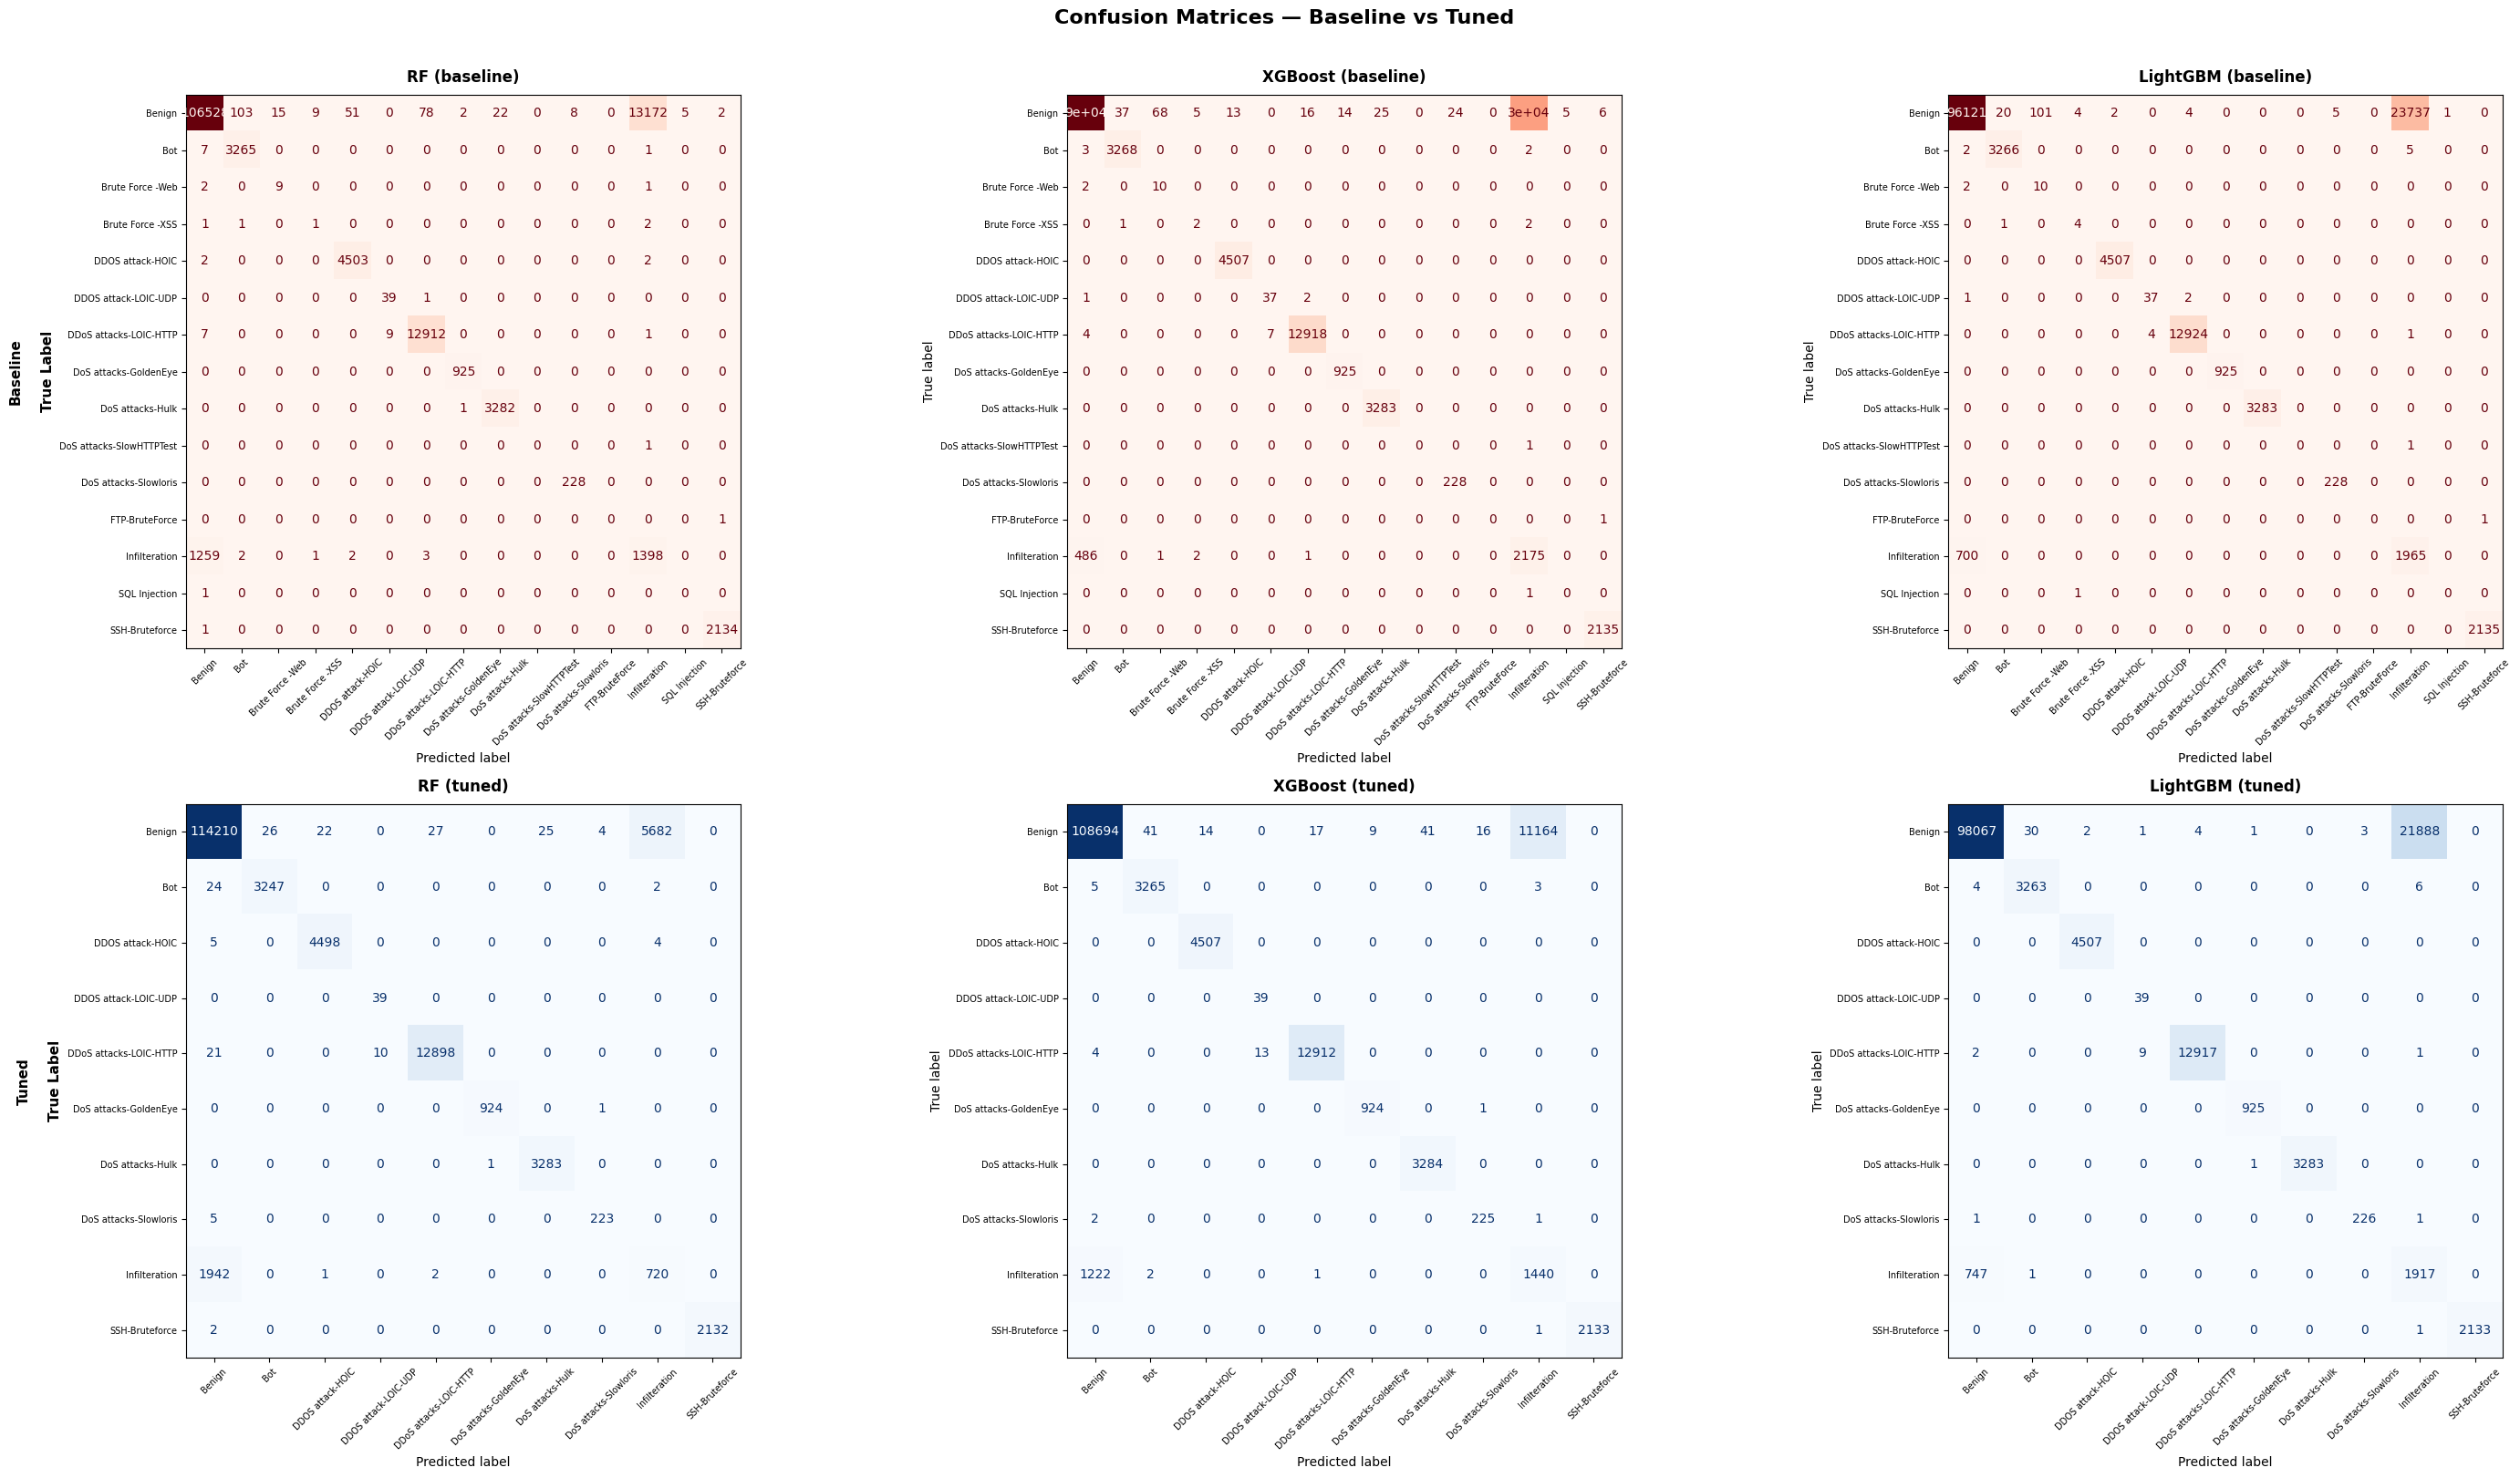
\includegraphics[width=\textwidth]{figures/confusion_matrices_all6.png}
  \caption{Matrices de confusion des modèles classiques : de base (en haut) vs. ajustés (en bas)}
  \label{fig:cic_ml_cm}
\end{figure}

%=============================================================================
\chapter{Apprentissage Profond et Architectures Hybrides}
\label{chap:dl}
%=============================================================================

Trois architectures de réseaux neuronaux ont été évaluées sur les deux jeux de données : LSTM Bidirectionnel (BiLSTM), CNN 1D et MLP. Toutes utilisent un entraînement pondéré par classe. Quatre stratégies hybrides (deux par jeu de données) combinent les forces complémentaires des modèles basés sur les arbres et des réseaux de neurones.

\section{NSL-KDD --- Résultats de l'Apprentissage Profond}

\subsection{LSTM / RNN}

Un LSTM à deux couches (64 et 32 unités, dropout 0,3, sortie sigmoïde, entropie croisée binaire) atteint \textbf{79,9 \%} de précision avec 3 980 faux négatifs—mieux que le CNN seul au seuil par défaut, mais en deçà du Gradient Boosting classique.

\subsection{CNN 1D}

Un CNN à deux blocs (Conv1D-64, MaxPool, Conv1D-32, MaxPool, Dense-64, Dropout-0,3, sigmoïde) atteint \textbf{78,1 \%} au seuil par défaut de 0,5 avec 4 265 faux négatifs. L'ajout de poids explicites pour les classes et l'abaissement du seuil à 0,3 réduisent les FN à \textbf{3 831} (précision : 79,8 \%).

\subsection{XGBoost Seul (Référence)}

XGBoost seul (400 estimateurs, profondeur 6, lr 0,05, seuil 0,3) atteint \textbf{81,1 \%} avec seulement 277 faux positifs mais 3 972 faux négatifs, confirmant sa complémentarité avec le CNN : haute précision, moins de FP, mais des FN similaires.

\section{CSE-CIC-IDS2018 --- Résultats de l'Apprentissage Profond}

\subsection{CNN 1D (Ajusté avec Keras Tuner)}

Le CNN 1D ajusté (deux blocs Conv1D avec BatchNormalization, GlobalAveragePooling, Dense-128, Dropout-0,3) atteint \textbf{97,98 \%} de précision—la plus élevée de tous les modèles sur ce jeu de données (Tableau~\ref{tab:cic_cnn_report}, Figure~\ref{fig:cic_cnn_cm}).

\begin{table}[H]
\centering
\caption{CSE-CIC-IDS2018 --- Résultats par classe du CNN 1D (ensemble de test, 149 980 échantillons)}
\label{tab:cic_cnn_report}
\begin{tabular}{lcccc}
\toprule
\textbf{Classe} & \textbf{Précision} & \textbf{Rappel} & \textbf{F1} & \textbf{Support} \\
\midrule
Benign                    & 0,98 & 1,00 & 0,99 & 119 996 \\
Bot                       & 1,00 & 0,99 & 0,99 & 3 273 \\
DDOS attack-HOIC          & 0,99 & 1,00 & 1,00 & 4 507 \\
DDOS attack-LOIC-UDP      & 0,75 & 0,97 & 0,84 & 39 \\
DDoS attacks-LOIC-HTTP    & 0,99 & 1,00 & 1,00 & 12 929 \\
DoS attacks-GoldenEye     & 0,99 & 1,00 & 1,00 & 925 \\
DoS attacks-Hulk          & 0,99 & 1,00 & 0,99 & 3 284 \\
DoS attacks-Slowloris     & 0,83 & 0,98 & 0,90 & 228 \\
Infilteration             & 0,34 & 0,04 & 0,08 & 2 665 \\
SSH-Bruteforce            & 1,00 & 1,00 & 1,00 & 2 134 \\
\midrule
\textbf{Précision globale} & \multicolumn{4}{c}{\textbf{97,98 \%}} \\
Moyenne macro             & 0,89 & 0,90 & 0,88 & 149 980 \\
\bottomrule
\end{tabular}
\end{table}

\begin{figure}[H]
  \centering
  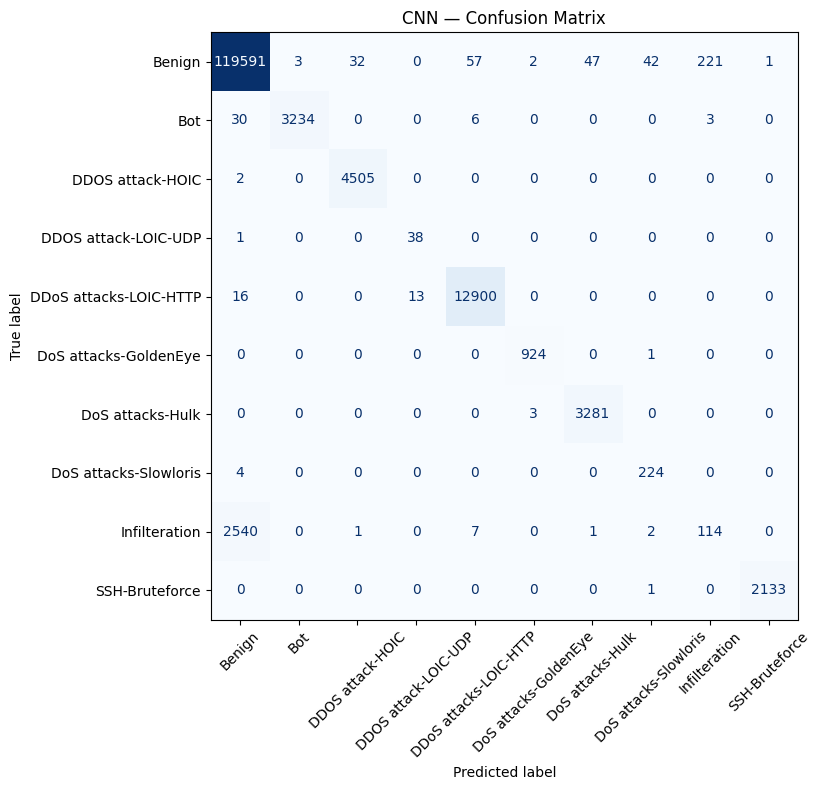
\includegraphics[width=0.55\textwidth]{figures/cic_cnn_cm.png}
  \caption{Matrice de confusion --- CNN 1D sur CSE-CIC-IDS2018}
  \label{fig:cic_cnn_cm}
\end{figure}

\subsection{LSTM Bidirectionnel}

Le BiLSTM n'atteint que \textbf{67,17 \%} de précision sur CSE-CIC-IDS2018—loin derrière tous les autres modèles. La précision de validation plafonne à 66--67 \% tandis que la perte de validation diverge.

\begin{infoorange}[Pourquoi le BiLSTM sous-performe sur les données IDS au niveau des flux]
Les caractéristiques de CSE-CIC-IDS2018 sont des \emph{agrégats statistiques} calculés sur l'ensemble des flux. Elles ne comportent aucun ordre temporel entre les dimensions des caractéristiques. Les injecter comme une séquence dans un LSTM gaspille la capacité sur des dépendances inexistantes et ajoute $\approx$33 s/époque de temps d'entraînement contre 1 s/époque pour le MLP.
\end{infoorange}

\subsection{Perceptron Multicouche (MLP)}

Le MLP (Dense-256, BatchNorm, Dropout-0,3, Dense-128, BatchNorm, Dropout-0,3, Dense-64, Dropout-0,2, Softmax) atteint \textbf{97,97 \%} de précision—virtuellement identique au CNN, mais s'entraîne en $\approx$1 s/époque. Du point de vue du déploiement, le MLP est préféré : une précision équivalente pour une fraction du temps d'entraînement.

\begin{table}[H]
\centering
\caption{Comparaison des modèles de réseaux de neurones sur CSE-CIC-IDS2018}
\label{tab:cic_nn_comparison}
\begin{tabular}{lccc}
\toprule
\textbf{Modèle} & \textbf{Précision de Test} & \textbf{Vitesse d'Entraînement} & \textbf{Notes} \\
\midrule
\rowcolor{lightgray}
\textbf{CNN 1D}  & \textbf{97,98 \%} & Moyenne & Le meilleur dans l'ensemble \\
MLP (DNN)        & 97,97 \%          & Rapide ($\approx$1s/ép.) & Presque identique au CNN \\
BiLSTM (RNN)     & 67,17 \%          & Lente ($\approx$33s/ép.) & Inéquation architecturale \\
\bottomrule
\end{tabular}
\end{table}

\section{Architectures d'Ensemble Hybrides}

\subsection{Hybride NSL-KDD 1 : XGBoost + CNN (Filtre en Cascade)}

XGBoost (seuil 0,25) signale les attaques probables, qui sont ensuite validées par le CNN. Résultat : 81,1 \% de précision, mais \textbf{4 069 FN}—\emph{plus} que XGBoost seul (3 972 FN). La deuxième étape conservatrice du CNN dégrade le rappel, confirmant que le filtrage séquentiel est contre-productif lorsque l'objectif est de minimiser les attaques manquées.

\subsection{Hybride NSL-KDD 2 : XGBoost + RF + MLP (Vote Souple Pondéré)}

Le vote souple (soft voting) sur trois modèles étalonnés (poids XGBoost 3, poids RF 1, poids MLP 1) avec un seuil $\tau = 0,25$ atteint \textbf{90,2 \%} de précision avec seulement \textbf{1 884 faux négatifs}—une amélioration spectaculaire par rapport à chaque modèle pris isolément. Un balayage systématique des seuils révèle le point de fonctionnement optimal à $\tau^* = 0,08$ : \textbf{2 954 FN} (30,7 \% de moins que le CNN par défaut), pour 347 faux positifs (Tableau~\ref{tab:nsl_threshold}, Figure~\ref{fig:nsl_threshold}).

\begin{table}[H]
\centering
\caption{Compromis FP/FN selon les seuils de décision $\tau$ (Ensemble hybride NSL-KDD)}
\label{tab:nsl_threshold}
\begin{tabular}{cccc}
\toprule
\textbf{Seuil $\tau$} & \textbf{FP} & \textbf{FN} & \textbf{TP} \\
\midrule
0,01 & 460 & 1 871 & 10 962 \\
0,05 & 367 & 2 525 & 10 308 \\
\rowcolor{lightgray}
\textbf{0,08} & \textbf{347} & \textbf{2 954} & \textbf{9 879} \\
0,10 & 334 & 3 066 & 9 767 \\
0,25 & 302 & 3 607 & 9 226 \\
0,30 & 292 & 3 732 & 9 101 \\
\bottomrule
\end{tabular}
\end{table}

\begin{figure}[H]
  \centering
  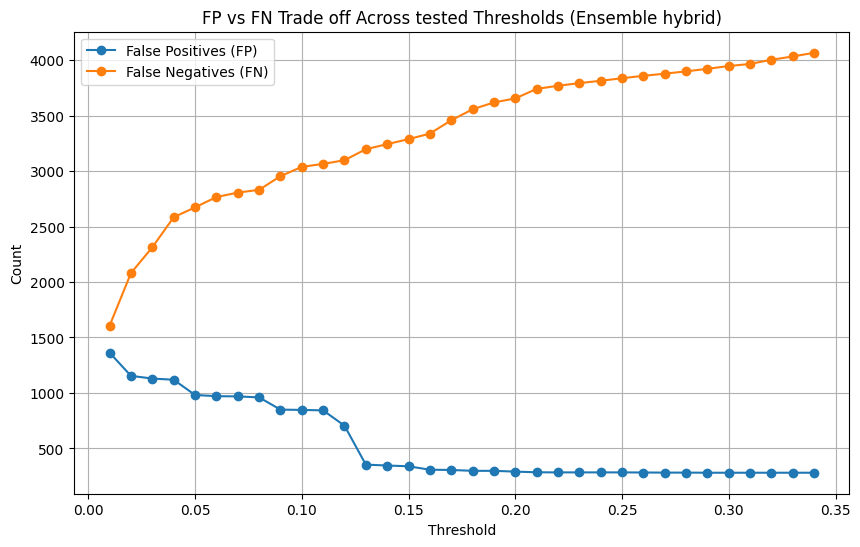
\includegraphics[width=0.65\textwidth]{figures/nsl_threshold_tradeoff.png}
  \caption{Courbe de compromis FP/FN pour l'ensemble NSL-KDD à travers les seuils de décision}
  \label{fig:nsl_threshold}
\end{figure}

\begin{figure}[H]
  \centering
  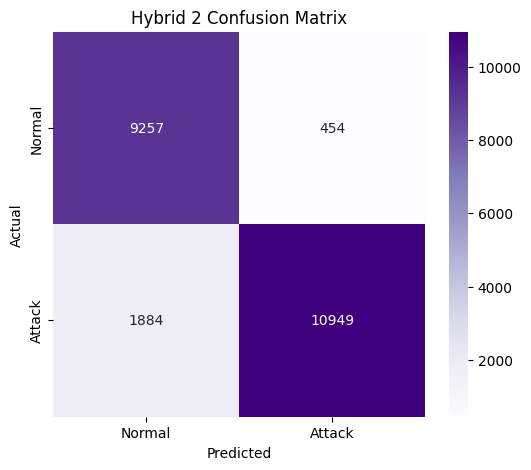
\includegraphics[width=0.55\textwidth]{figures/nsl_ensemble_cm.png}
  \caption{Matrice de confusion --- Ensemble XGB+RF+MLP sur NSL-KDD ($\tau = 0,25$)}
  \label{fig:nsl_ensemble_cm}
\end{figure}

\subsection{Hybride CSE-CIC-IDS2018 1 : XGBoost + CNN (Empilement de Caractéristiques)}

Les plongements de l'avant-dernière couche du CNN (128-dim) sont concaténés avec les vecteurs de probabilité de classe de XGBoost (10-dim) et transmis à une méta-tête. L'hybride atteint \textbf{97,89 \%}—légèrement en dessous du CNN seul (97,98 \%). L'entraînement s'achève en moins de deux minutes, ce qui en fait une alternative pratique.

\subsection{Hybride CSE-CIC-IDS2018 2 : XGBoost + RF + MLP (Ensemble d'Empilement)}

Les sorties de probabilité de classe de XGBoost, RF et MLP (30-dim combinés) alimentent une méta-tête plus profonde. Malgré la combinaison de trois modèles, la précision tombe à \textbf{96,43 \%} : XGBoost et RF partagent des modèles d'erreur corrélés sur la classe Infiltration, et la méta-tête ne peut pas corriger les défaillances partagées systématiques.

\begin{table}[H]
\centering
\caption{Comparaison des modèles hybrides sur CSE-CIC-IDS2018}
\label{tab:cic_hybrid_comp}
\begin{tabular}{lcc}
\toprule
\textbf{Hybride} & \textbf{Précision} & \textbf{Notes} \\
\midrule
XGB + CNN (stacking de caractéristiques) & 97,89 \% & Rapide ($<$2 min), perf. proche du CNN \\
XGB + RF + MLP (stacking)    & 96,43 \% & Les erreurs corrélées limitent l'amélioration \\
\bottomrule
\end{tabular}
\end{table}

\section{Analyse Comparative}

Le Tableau~\ref{tab:final_summary} consolide l'ensemble des résultats. Aucun modèle ne domine sur les deux jeux de données : l'ensemble XGB+RF+MLP est en tête sur NSL-KDD (90,2 \%), tandis que le CNN autonome domine sur CSE-CIC-IDS2018 (97,98 \%).

\begin{table}[H]
\centering
\caption{Résumé complet des performances à travers tous les modèles et jeux de données}
\label{tab:final_summary}
\footnotesize
\setlength{\tabcolsep}{4pt}
\begin{tabularx}{\textwidth}{@{}>{\raggedright\arraybackslash}p{4.2cm} >{\centering\arraybackslash}p{2.1cm} >{\centering\arraybackslash}p{2.1cm} X@{}}
\toprule
\textbf{Modèle / Approche} & \textbf{NSL-KDD} & \textbf{CIC-IDS2018} & \textbf{Notes} \\
\midrule
\rowcolor{lightgray}
\textbf{XGB+RF+MLP} ($\tau{=}0,25$) & \textbf{90,2 \%} & 96,43 \% & Meilleure précision NSL ; 1 884 FN \\
XGBoost (ajusté) & 81,1 \% & 91,63 \% & Moins de FP sur NSL (277) \\
XGB + CNN & 81,1 \% & 97,89 \% & Cascade (NSL) ; stacking (CIC) \\
Gradient Boosting & 80,6 \% & --- & Meilleur F1 sur NSL (0,800) \\
BiLSTM / RNN & 79,9 \% & 67,17 \% & Inéquation architecturale sur CIC \\
CNN 1D (ajusté) & 79,8 \% & \textbf{97,98 \%} & Meilleure précision CIC \\
Random Forest (ajusté) & 78,1 \% & 94,80 \% & Meilleur classique sur CIC \\
MLP / DNN & --- & 97,97 \% & Quasi-égalité avec le CNN sur CIC \\
LightGBM (ajusté) & --- & 84,86 \% & Score CIC ajusté le plus bas \\
\bottomrule
\multicolumn{4}{@{}l@{}}{\small À $\tau^*{=}0,08$, XGB+RF+MLP donne FN\,=\,2 954 sur NSL-KDD (30,7 \% de moins que le CNN par défaut).} \\
\end{tabularx}
\end{table}

\begin{figure}[H]
  \centering
  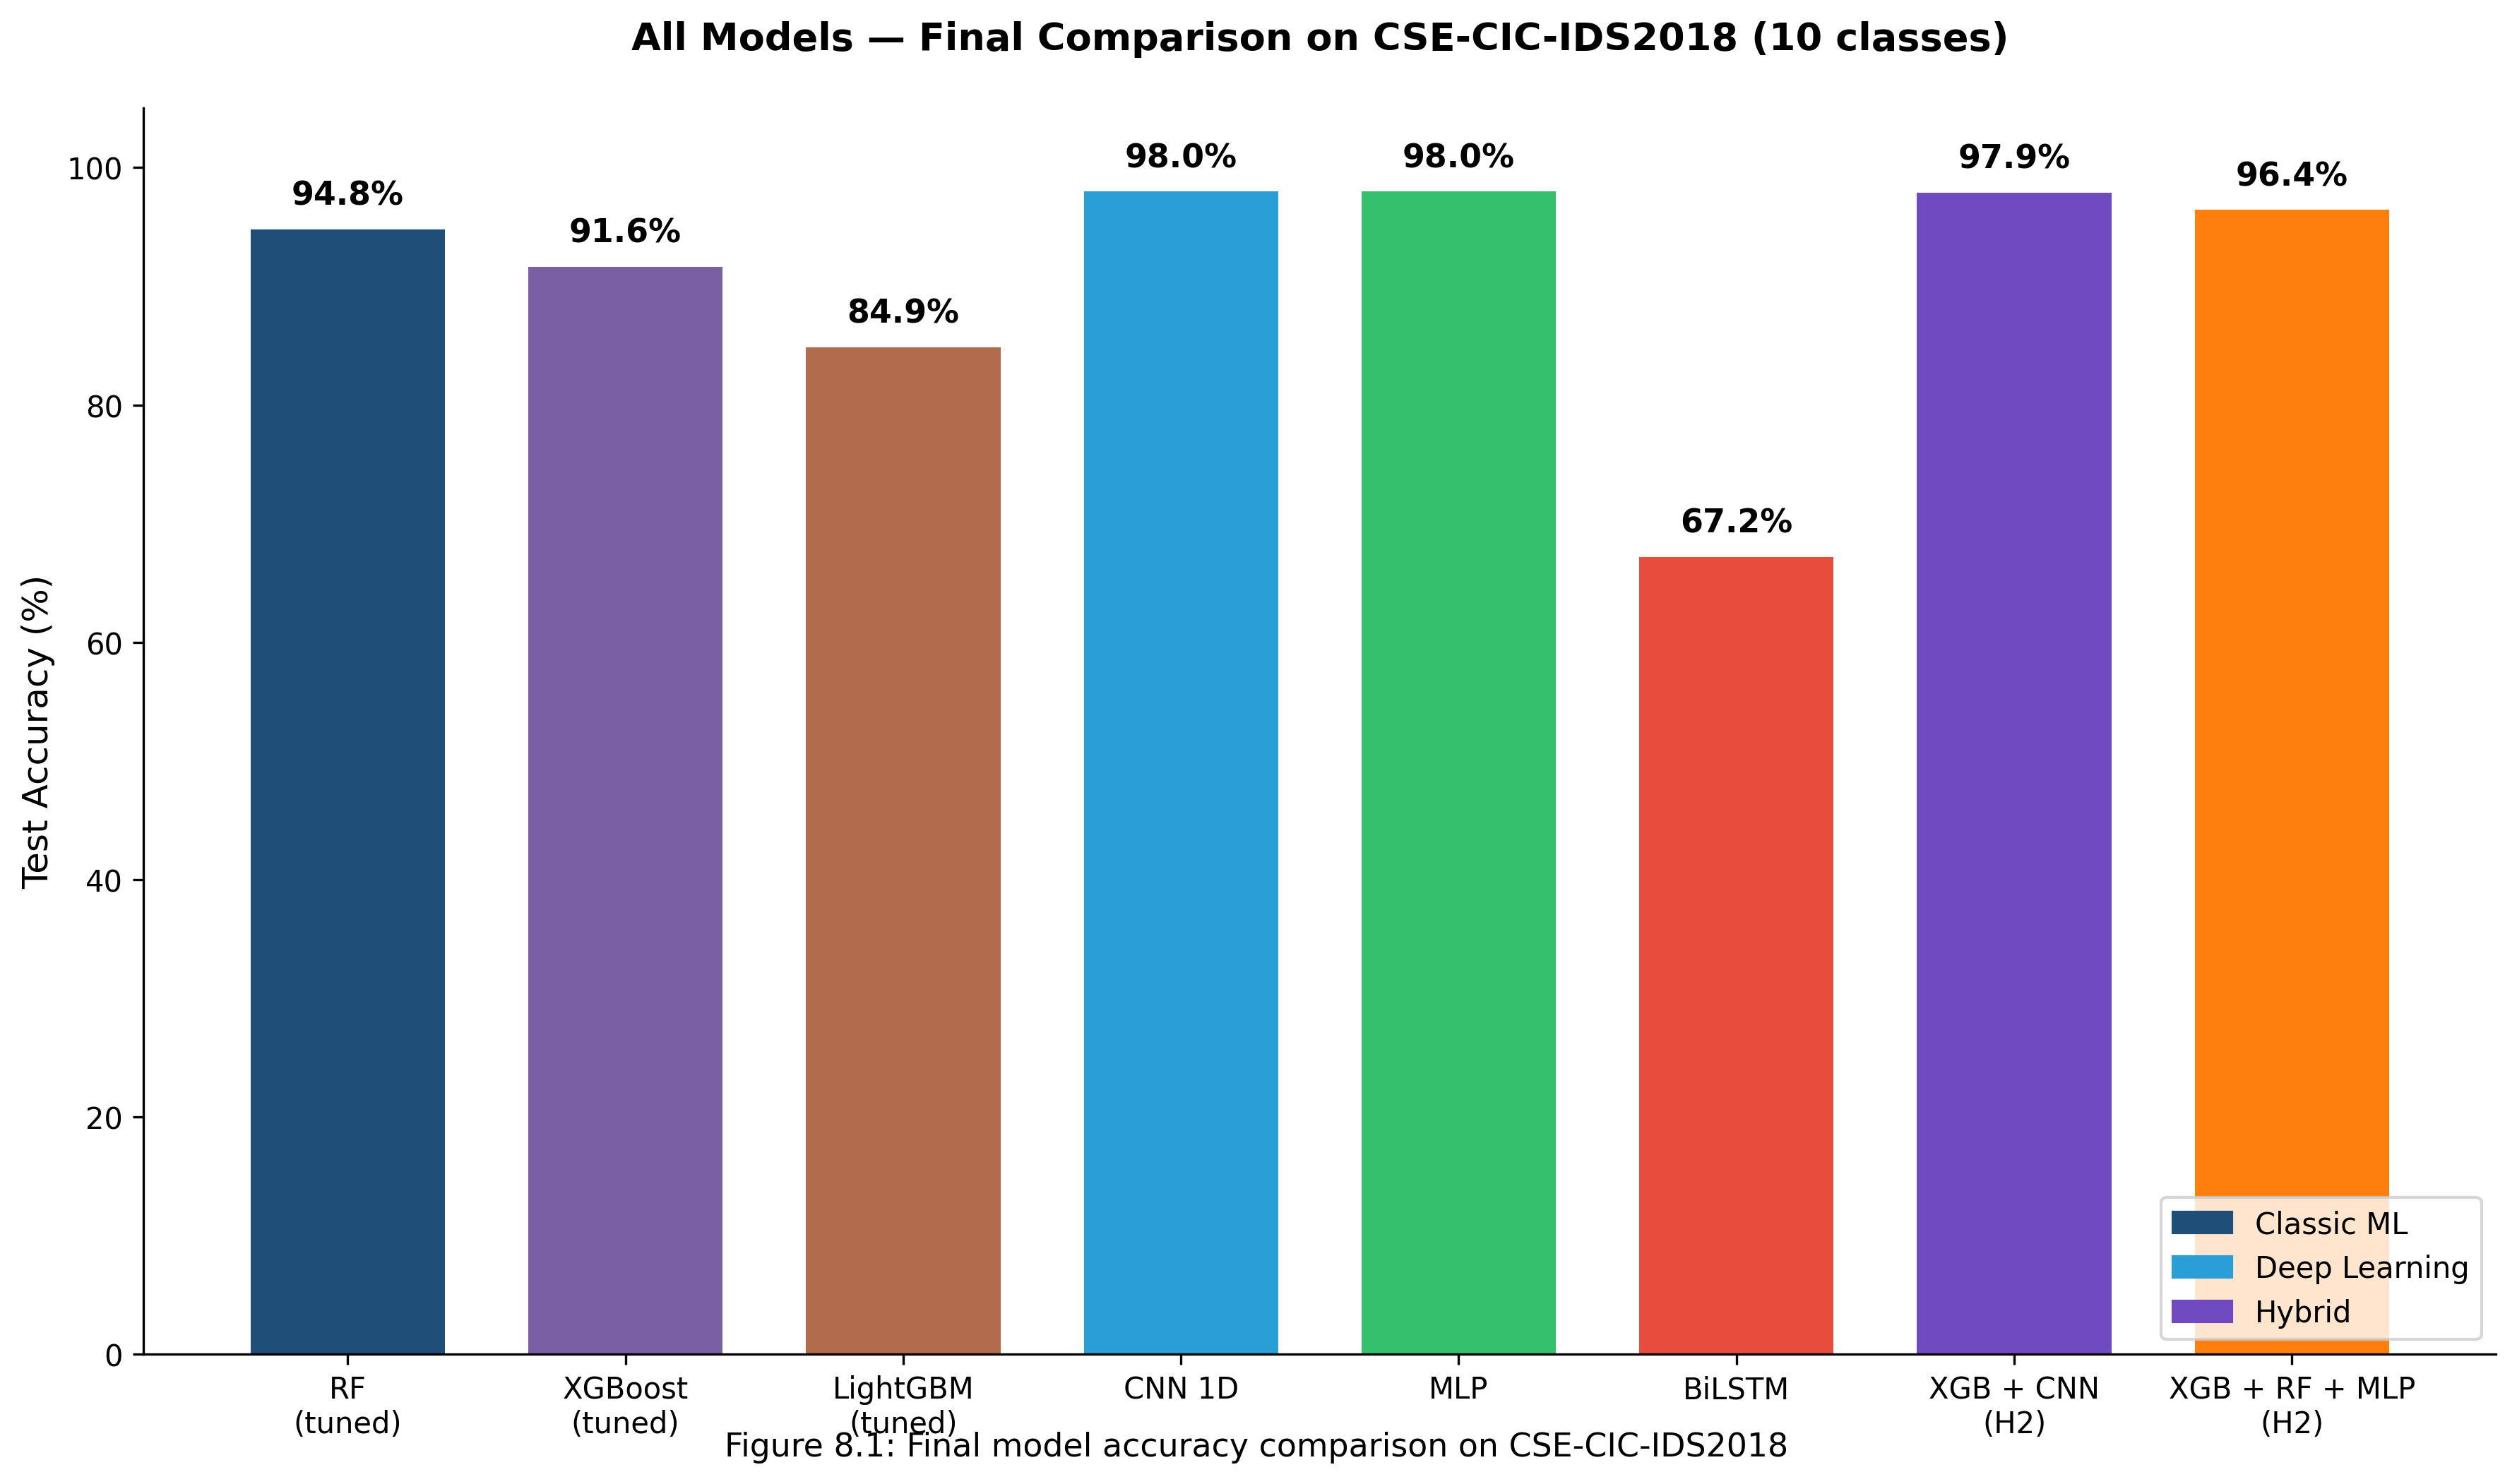
\includegraphics[width=\textwidth]{figures/cic_final_comparison.png}
  \caption{Comparaison de la précision finale des modèles sur CSE-CIC-IDS2018}
  \label{fig:cic_final}
\end{figure}

\begin{figure}[H]
  \centering
  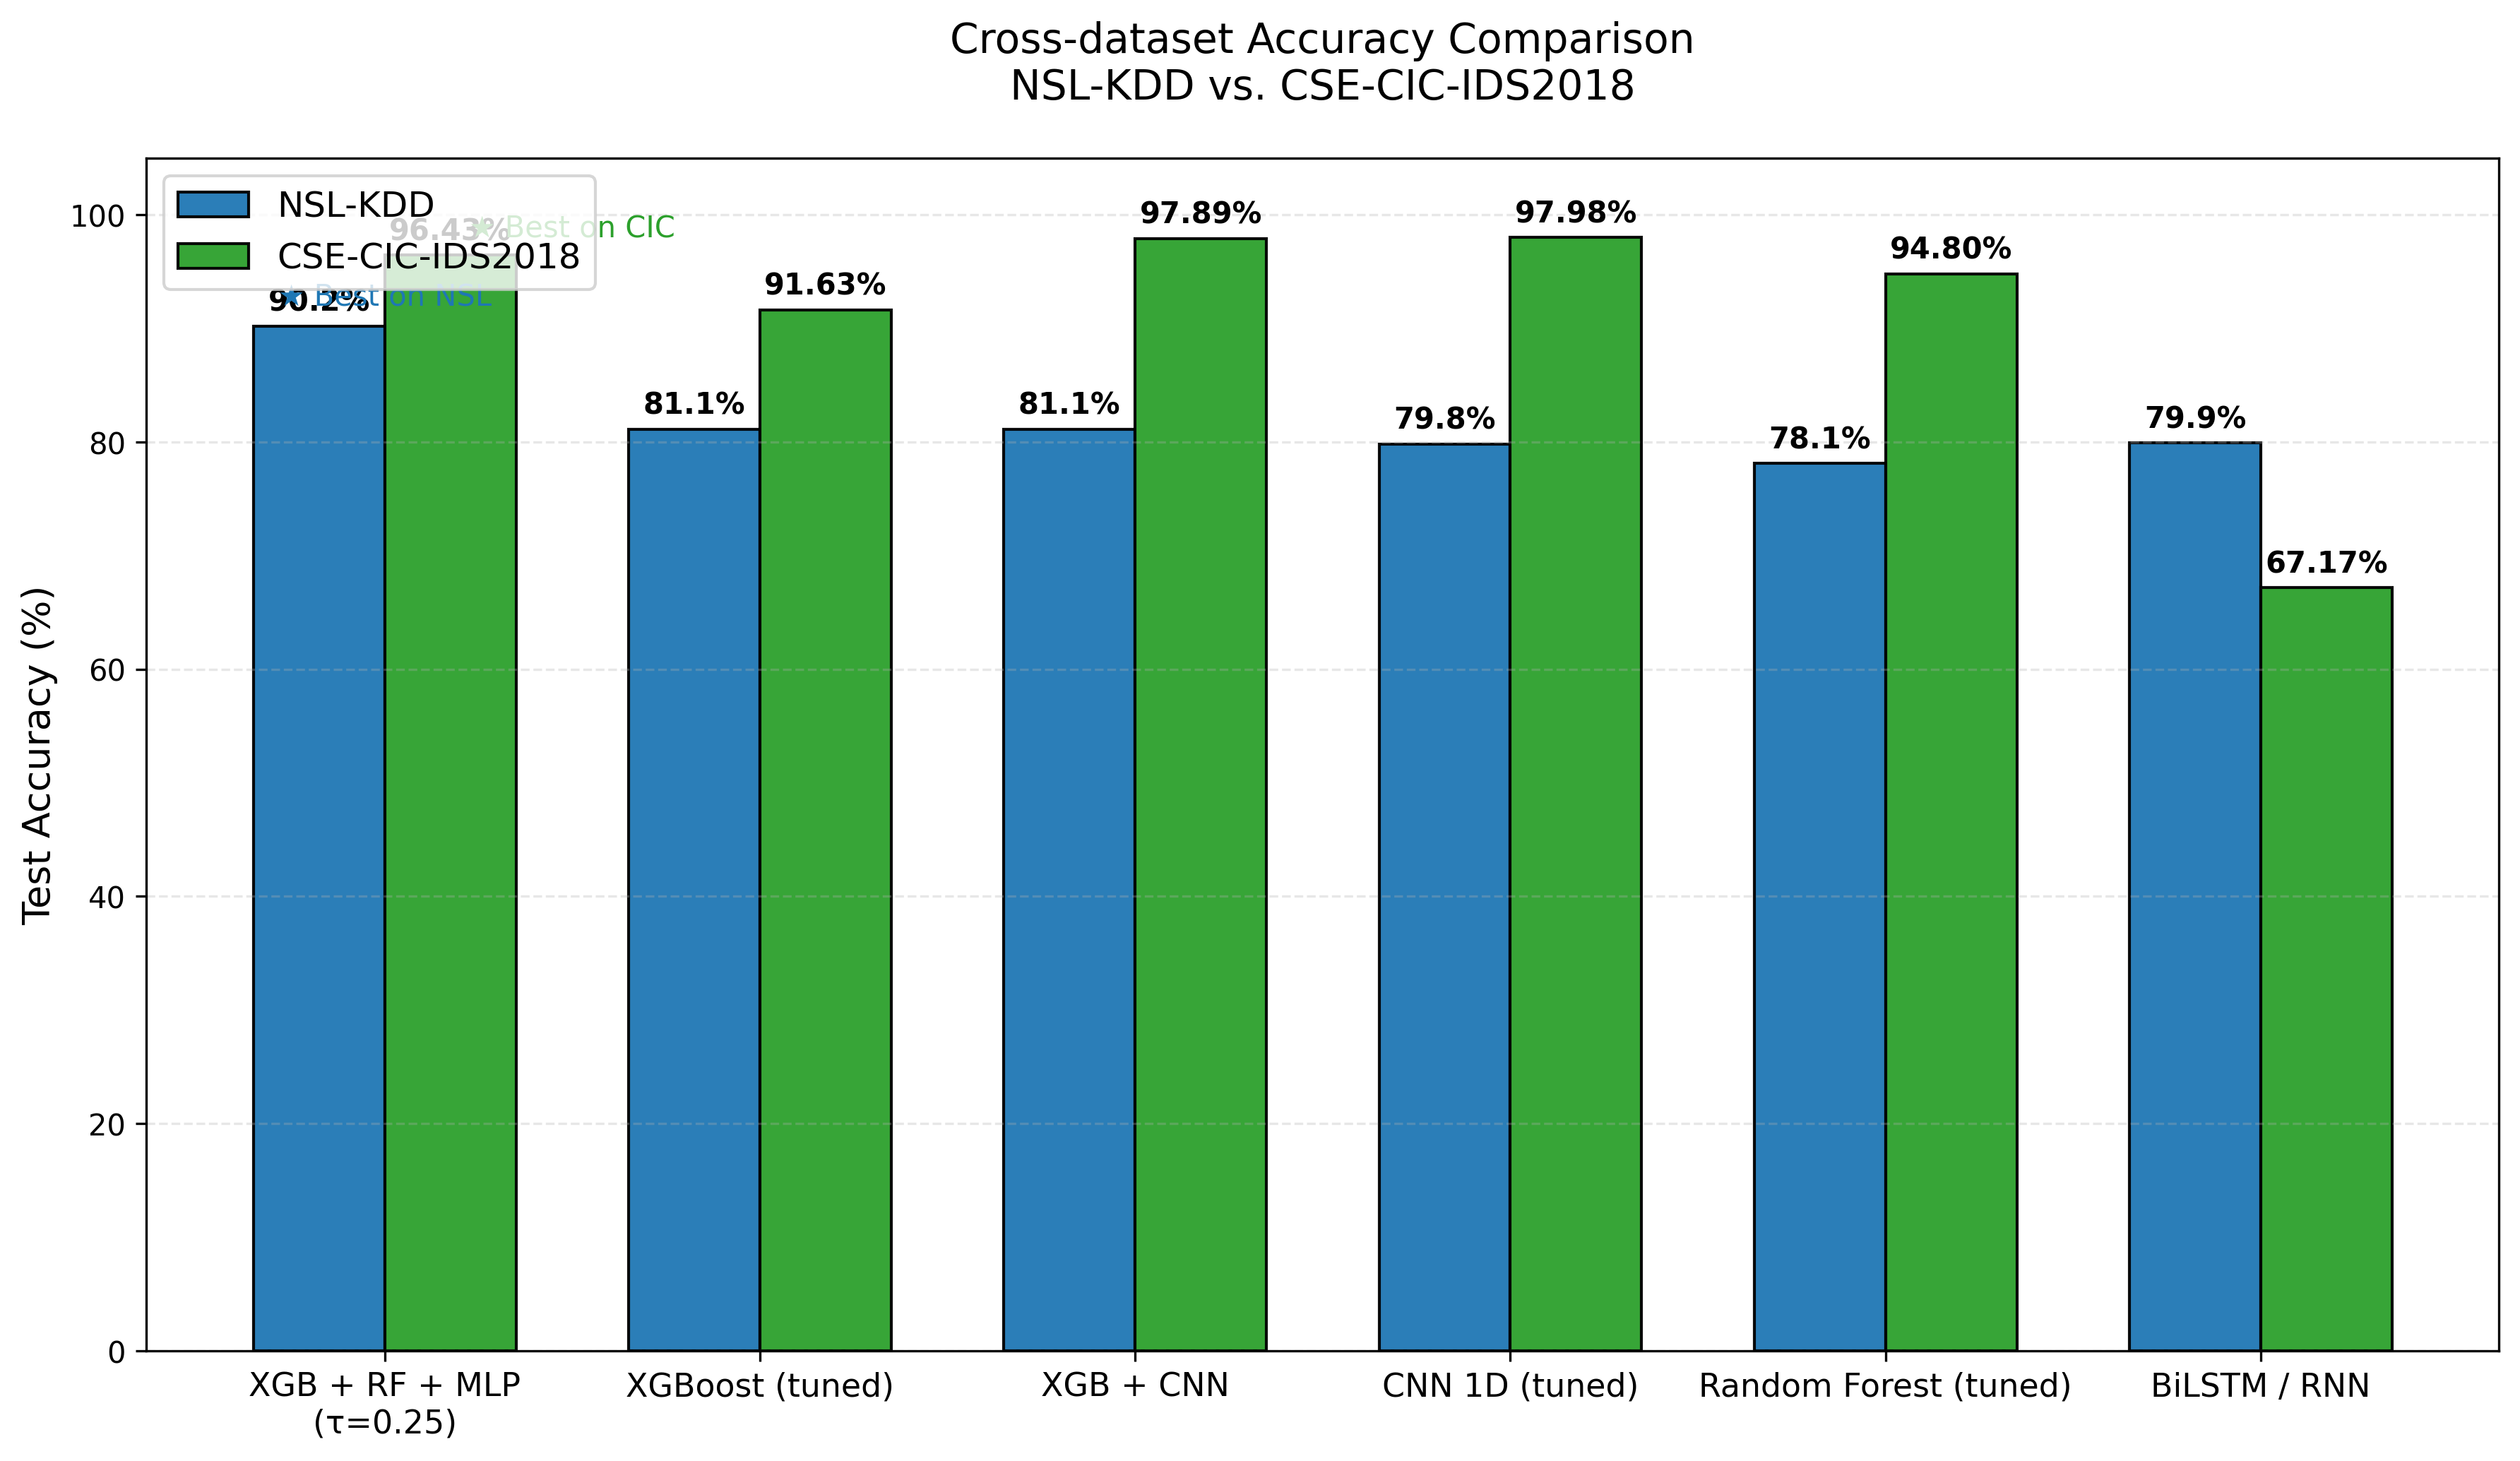
\includegraphics[width=\textwidth]{figures/cross_dataset_comparison.png}
  \caption{Comparaison de la précision inter-jeux de données : NSL-KDD vs. CSE-CIC-IDS2018}
  \label{fig:cross_dataset}
\end{figure}

%=============================================================================
\chapter{General Conclusion}
\label{chap:general_conclusion}
%=============================================================================

\section{Principal Findings}

\textbf{Dataset scale and feature richness drive performance.} All model families improve systematically from NSL-KDD to CSE-CIC-IDS2018: classical ensembles from 78--81\% to 85--95\%, deep learning from 78--80\% to 97--98\%. The richer 77-feature CICFlowMeter set and larger training volume explain this jump.

\textbf{Accuracy alone is insufficient.} On NSL-KDD, the XGB+RF+MLP ensemble at $\tau{=}0.25$ achieves 90.2\% accuracy with only 1,884 FN—proving that architecture, calibration, and threshold together can improve both metrics simultaneously. Confusion matrices must always complement accuracy numbers.

\textbf{Architectural fit matters more than complexity.} The BiLSTM's collapse to 67.17\% on CIC is not a failure of deep learning (CNN and MLP achieve 97--98\%). LSTM gating mechanisms require temporally ordered sequences, but flow features are statistical aggregates with no meaningful intra-vector ordering.

\textbf{Class imbalance management is non-negotiable.} Adding class weights and lowering the CNN threshold from 0.5 to 0.3 reduces false negatives from 4,265 to 3,831. The systematic threshold sweep on the ensemble reduces FN from 3,607 ($\tau{=}0.25$) to 2,954 ($\tau{=}0.08$)—an 18.1\% further improvement.

\textbf{Hybrid strategy matters more than hybrid count.} The XGB+RF+MLP soft-voting ensemble outperforms the XGB+CNN cascade (1,884 vs.\ 4,069 FN) because the cascade degrades XGBoost's recall. Adding more models without ensuring error diversity can worsen results.

\textbf{The Infiltration problem remains open.} Per-class recall for Infiltration is consistently 0.04--0.21 across all evaluated models (F1 = 0.08--0.17). These attacks deliberately mimic benign traffic, generating only minimal statistical deviations in flow-level features. Solving Infiltration detection likely requires longer time-window analysis or packet-level payload features beyond single-flow aggregates.

\section{Perspectives and Future Work}

\paragraph{Multi-class NSL-KDD.} Extending NSL-KDD experiments to 5-class (Normal + DoS, Probe, R2L, U2R) with SMOTE or few-shot techniques for the rare R2L and U2R classes.

\paragraph{Attention mechanisms and transformers.} TabTransformer and FT-Transformer have shown strong results on structured data; their application to Infiltration detection merits exploration.

\paragraph{Online and continual learning.} Static batch-trained models degrade as attack patterns evolve. Incremental learning frameworks that update parameters on incoming traffic are critical for operational deployment.

\paragraph{Generalisation across environments.} Transfer learning and domain-adversarial training across IDS datasets from different network contexts could directly address the dataset bias problem.

\paragraph{Graph-based anomaly detection.} Traffic has an inherent graph structure (hosts as nodes, flows as edges). Graph Neural Networks may capture structural attack patterns (e.g., port-scanning topologies) invisible to flow-level classifiers.

This study demonstrates that effective AI-based intrusion detection demands careful attention to dataset characteristics, preprocessing rigour, architectural suitability, and operational threshold design. The XGB+RF+MLP ensemble and the 1D CNN are the best practical choices for binary and multi-class IDS deployments respectively. The Infiltration challenge points toward richer feature representations and more advanced architectures as productive future directions.

%─── Bibliography ─────────────────────────────────────────────────────────────
\begin{thebibliography}{99}

\bibitem{tavallaee2009}
M.~Tavallaee, E.~Bagheri, W.~Lu, A.~A.~Ghorbani,
\textit{A Detailed Analysis of the KDD CUP 99 Data Set},
in \textit{Proc. IEEE Symposium on Computational Intelligence for Security and Defense Applications (CISDA)}, 2009, pp. 1--6.

\bibitem{sharafaldin2018}
I.~Sharafaldin, A.~H.~Lashkari, A.~A.~Ghorbani,
\textit{Toward Generating a New Intrusion Detection Dataset and Intrusion Traffic Characterization},
in \textit{Proc. 4th International Conference on Information Systems Security and Privacy (ICISSP)}, 2018, pp. 108--116.

\bibitem{goodfellow2016}
I.~Goodfellow, Y.~Bengio, A.~Courville,
\textit{Deep Learning},
MIT Press, Cambridge, MA, 2016.

\bibitem{scikit}
F.~Pedregosa \textit{et al.},
\textit{Scikit-learn: Machine Learning in Python},
\textit{Journal of Machine Learning Research}, vol.~12, pp.~2825--2830, 2011.

\bibitem{tensorflow}
M.~Abadi \textit{et al.},
\textit{TensorFlow: A System for Large-Scale Machine Learning},
in \textit{Proc. 12th USENIX Symposium on Operating Systems Design and Implementation (OSDI)}, 2016, pp.~265--283.

\end{thebibliography}

\end{document}
